\subsection{Conceptual introduction}
\begin{frame}
\frametitle{sets}
\begin{center}	
			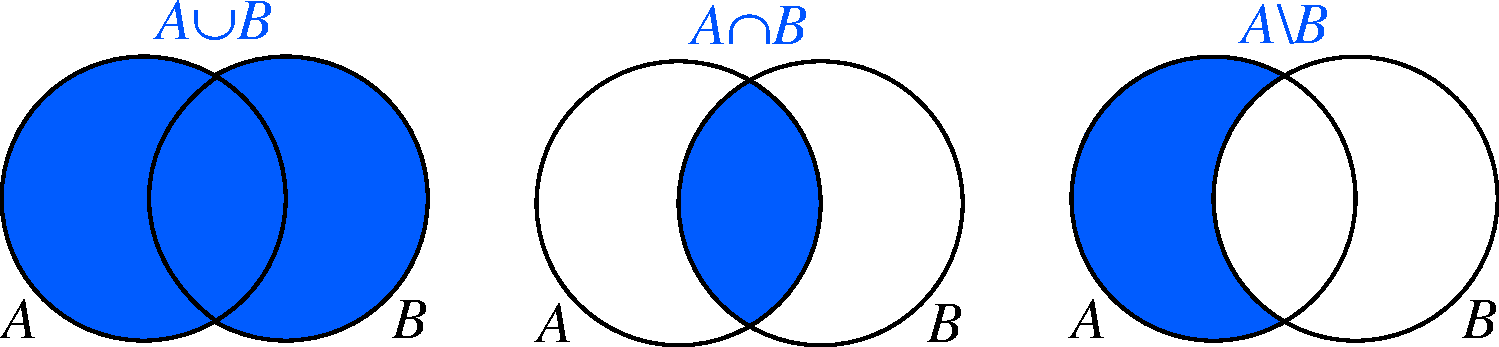
\includegraphics[scale=0.45]{fig/setth.pdf}
	\end{center}		
\end{frame}

\begin{frame}
\frametitle{probability measure}
\begin{center}	
			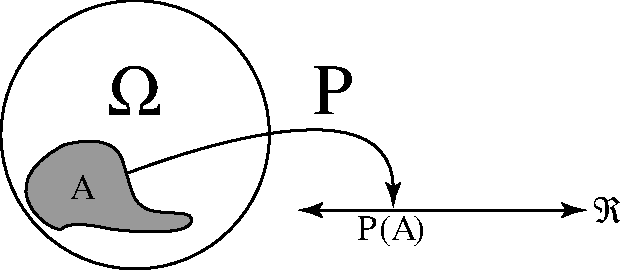
\includegraphics[scale=0.45]{fig/propmeas5.pdf}
	\end{center}		
\end{frame}

\begin{frame}
\frametitle{probability axioms}
\begin{center}	
			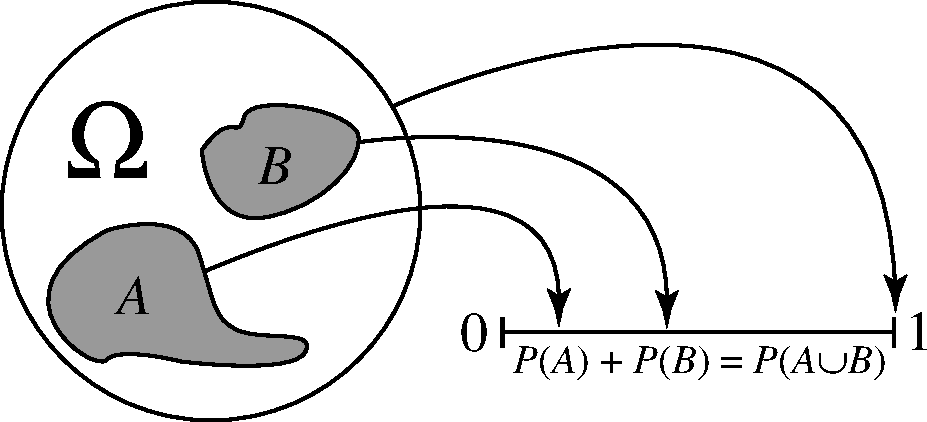
\includegraphics[scale=0.45]{fig/probthax7.pdf}
	\end{center}		
\end{frame}

\begin{frame}
\frametitle{conditional probability}
\begin{center}	
			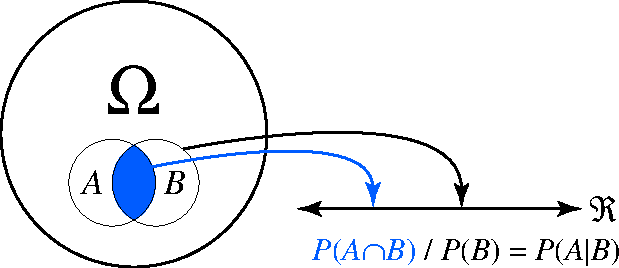
\includegraphics[scale=0.45]{fig/condprob10.pdf}
	\end{center}		
\end{frame}

\begin{frame}
\frametitle{random variables}
\begin{center}	
			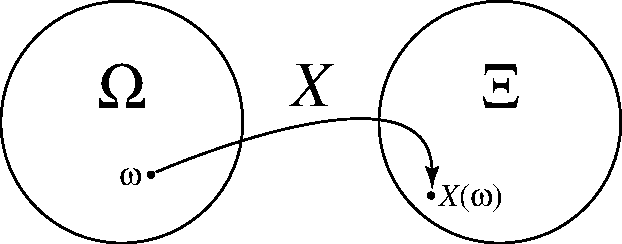
\includegraphics[scale=0.45]{fig/randvar15.pdf}
	\end{center}		
\end{frame}

\begin{frame}
\frametitle{probability densities}
\begin{center}	
			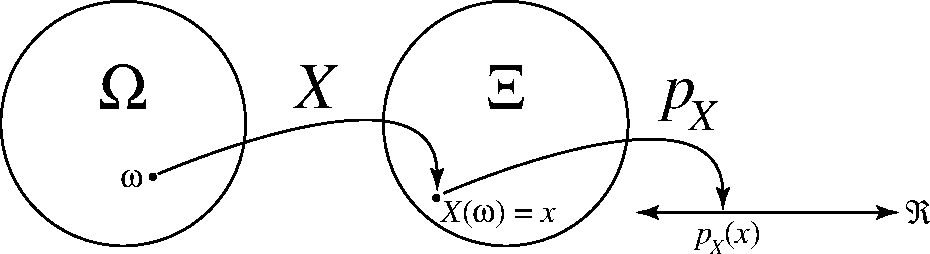
\includegraphics[scale=0.45]{fig/probdensity17.pdf}
	\end{center}		
\end{frame}

\begin{frame}
\frametitle{joint probability densities}
\begin{center}	
			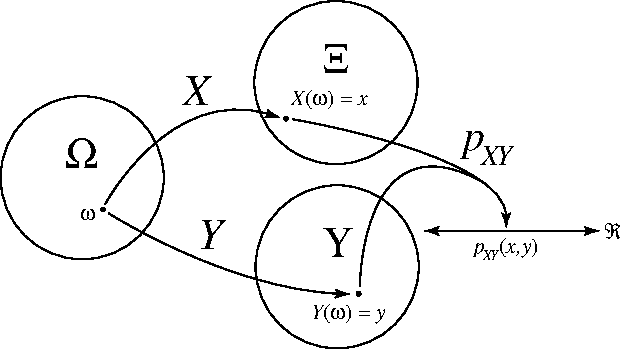
\includegraphics[scale=0.45]{fig/probjointdens18.pdf}
	\end{center}		
\end{frame}

\begin{frame}
\frametitle{the reality}
\begin{center}	
			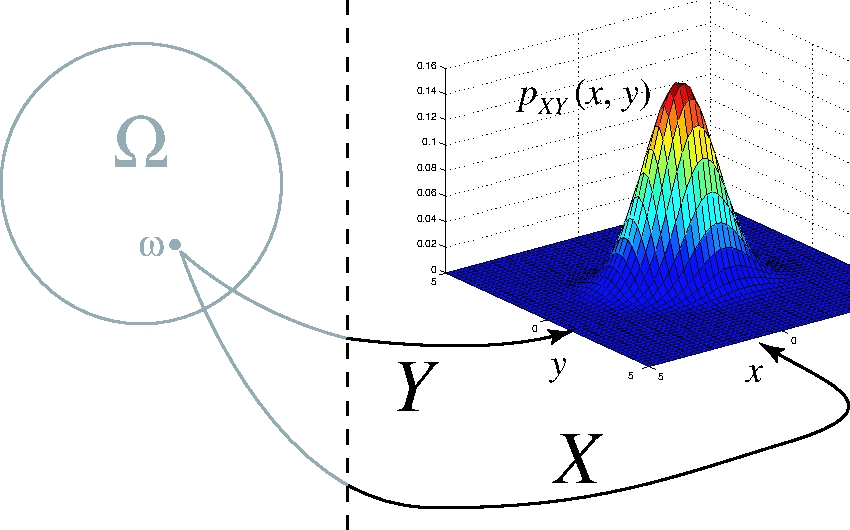
\includegraphics[scale=0.45]{fig/probreality19.pdf}
	\end{center}		
\end{frame}

\subsection{Measure theory}
\begin{frame}
\begin{itemize}
\item For the general theory of measure spaces, we first need a \emph{measurable space} $(X, \Sigma)$, that is a set equipped with a collection $\Sigma$ of \textbf{measurable sets} complete under certain operations. Then this becomes a measure space $(X, \Sigma, \mu)$ by throwing in a function $\mu$ from $\Sigma$ to a space of values (such as the real line) that gets along with the set-theoretic operations that $\Sigma$ has. If $E$ is a measurable set, then $\mu(E)$ is called the \textbf{measure} of $E$ with respect to $\mu$. \cite{Houle2011}
\end{itemize}
\end{frame}

\begin{frame}
\begin{enumerate}
\item Given a set $X$, 
\item a \textbf{$\sigma$-algebra} is a collection of subsets of $X$ that is closed under complementation, countable unions, and countable intersections. 
\item A \textbf{measurable space}, by the usual modern definition, is a set $X$ equipped with a $\sigma$-algebra $\Sigma$. 
\item The elements of $\Sigma$ are called the \textbf{measurable sets} of $X$ (or more properly, the measurable subsets of $(X,\Sigma)$). \cite{Teh2006}
\end{enumerate}
\end{frame}

\begin{frame}
A \textbf{measure space} is a \textbf{measurable space} equipped with a \textbf{measure}. There are many different types of measures parametrized by the type of their codomains. Let $(X, \Sigma)$ be a measurable space. A \textbf{probability measure} on $X$ (due to Kolmogorov) is a function $\mu$ from the collection $\Sigma$ of measurable sets to the unit interval $[0,1]$ such that:

\begin{enumerate}%
\item The measure of the empty set is zero: $\mu(\emptyset) = 0$;
\item The measure of the entire space is one: $\mu(X) = 1$;
\item Countable additivity: $\mu(\bigcup_{i = 1}^{\infty} S_i) = \sum_{i=1}^{\infty} \mu(S_i)$ whenever the $S_i$ are mutually disjoint sets|disjoint.
(Part of the latter condition is the requirement that the sum on the right-hand side must converge.)
\end{enumerate}
\end{frame}

\begin{frame}
It is sometimes stated (but in fact follows from the previous) that:

\begin{itemize}%
\item Finitary additivity: $\mu(S \cup T) = \mu(S) + \mu(T)$ whenever $S$ and $T$ are disjoint.
\item $\mu$ is increasing: $\mu(A) \leq \mu(B)$ if $A \subseteq B$.

\end{itemize}
\end{frame}

%\begin{frame}
%\begin{itemize}
%\item Let $\Omega$ be a set.
%\item Let $\cal{F}$ be a $\sigma$-algebra of subsets of $\Omega$.
%\item Let $\textbf{P}:\cal{F} \rightarrow$ $[0, 1]$ be a measure on $\Omega$ s.t. $\textbf{P}(\Omega) =1$. 
%\end{itemize}
%
%\textbf{Definition:} $(\Omega, \cal{F}, \textbf{P})$ is called a \textbf{probability space} \cite{Houle2011}.\\
%
%Let $X : \Omega \rightarrow \mathbb{R}$  be an $\cal{F}$-measurable function.
%
%i.e., $X^{-1}(A) \in {\cal {F}}$ $\forall A \in \cal B$
%
%We say $X$ is a \textbf{random variable}.\\
%
%\textbf{Definition:} If X is integrable (i.e.\ $\int |X|\; d\textbf{P} < \infty$), then define 
%$$\textbf{E}(X) = \int X\; d\textbf{P}.$$ \cite{Teh2006}
%
%An element of $\cal{F}$ is called an \textbf{event}.  
%
%Two events $A$ and $B$ are said to be \textbf{independent} if $\textbf{P}(A \cap B) = \textbf{P}(A) \textbf{P}(B)$.
%\end{frame}
%
%\subsection{Probability theory}
%\begin{frame}
%
%\textbf{Example:} Toss a fair coin. Observe 1 of 2 outcomes: Heads or Tails.
%
%Construct the following probability space.
%
%\begin{itemize}
%\item $\Omega = \{H,T\}$
%\item ${\cal F} = \{\phi, H, T, \Omega\}$
%\end{itemize}
%
%Define a probability on $\cal{F}$:\\
%$\textbf{P}(\phi)=0$, $\textbf{P}(H) = \frac{1}{2} = \textbf{P}(T)$, $\textbf{P}(\Omega)=1$
%
%Define the rv $X$ to be outcome of toss:\\
%$X=x$ where $x \in \{H,T\}$
%
%Repeatedly toss this coin.  
%
%Let $\{X_{j}\}$, $j = 0,1,2,\dots$ be a collection of rv's s.t. $\textbf{P}(X_{j}=H) = \frac{1}{2} = \textbf{P}(X_{j}=T)$.
%
%\end{frame}